%; whizzy paragraph -pdf xpdf -latex ./whizzypdfptex.sh
%; whizzy-paragraph "^\\\\begin{frame}\\|\\\\emtext"
% latex beamer presentation.
% platex, latex-beamer でコンパイルすることを想定。 

%     Tokyo Debian Meeting resources
%     Copyright (C) 2012 Junichi Uekawa
%     Copyright (C) 2016 Nobuhiro Iwamatsu

%     This program is free software; you can redistribute it and/or modify
%     it under the terms of the GNU General Public License as published by
%     the Free Software Foundation; either version 2 of the License, or
%     (at your option) any later version.

%     This program is distributed in the hope that it will be useful,
%     but WITHOUT ANY WARRANTY; without even the implied warreanty of
%     MERCHANTABILITY or FITNESS FOR A PARTICULAR PURPOSE.  See the
%     GNU General Public License for more details.

%     You should have received a copy of the GNU General Public License
%     along with this program; if not, write to the Free Software
%     Foundation, Inc., 51 Franklin St, Fifth Floor, Boston, MA  02110-1301 USA

\documentclass[cjk,dvipdfmx,12pt]{beamer}
\usetheme{Tokyo}
\usepackage{monthlypresentation}

%  preview (shell-command (concat "evince " (replace-regexp-in-string "tex$" "pdf"(buffer-file-name)) "&")) 
%  presentation (shell-command (concat "xpdf -fullscreen " (replace-regexp-in-string "tex$" "pdf"(buffer-file-name)) "&"))
%  presentation (shell-command (concat "evince " (replace-regexp-in-string "tex$" "pdf"(buffer-file-name)) "&"))

%http://www.naney.org/diki/dk/hyperref.html
%日本語EUC系環境の時
\AtBeginDvi{\special{pdf:tounicode EUC-UCS2}}
%シフトJIS系環境の時
%\AtBeginDvi{\special{pdf:tounicode 90ms-RKSJ-UCS2}}

\newenvironment{commandlinesmall}%
{\VerbatimEnvironment
  \begin{Sbox}\begin{minipage}{1.0\hsize}\begin{fontsize}{8}{8} \begin{BVerbatim}}%
{\end{BVerbatim}\end{fontsize}\end{minipage}\end{Sbox}
  \setlength{\fboxsep}{8pt}
% start on a new paragraph

\vspace{6pt}% skip before
\fcolorbox{dancerdarkblue}{dancerlightblue}{\TheSbox}

\vspace{6pt}% skip after
}
%end of commandlinesmall

\title{東京エリアDebian勉強会\\Debian JP Project}
\subtitle{OSC 2017 Tokyo/Fall (第154回出張勉強会)}
\author{杉本 典充\\ dictoss@live.jp}
\date{2017年09月10日}
\logo{
\includegraphics[width=8cm]{image200607/openlogo-light.eps}}

\begin{document}

\begin{frame}
\titlepage{}
\end{frame}

\begin{frame}{Agenda}
  \begin{itemize}
  \item Debian とは?
  \item Debian 9 情報
  \item Debian Updates
  \item 今後のイベント
  \end{itemize}
\end{frame}

%-------------------

\section{Debian とは?}
\begin{frame}\begin{center}\Huge{Debian とは?}\end{center}\end{frame}


\begin{frame}{Debian とは?}

{\color{red}{フリー/オープン}}な{\color{red}{ユニバーサル}}オペレーティングシステム を作成しようとするボランティアベースのプロジェクト。

\begin{table}[htb]
  \begin{tabular}{|c|c|c|}
    \hline
    ディストリ & 企業 & ボランティア \\ \hline
    RHEL & RedHat & なし  \\ \hline
    CentOS & RedHat & あり \\ \hline
    Ubuntu  & Canonical & あり \\ \hline
    \color{red}{Debian}  & \color{red}{なし} & \color{red}{あり} \\ \hline
  \end{tabular}
\end{table}

\end{frame}


\begin{frame}{Debian とは?}
Linux カーネルだけではなく、FreeBSD や GNU/Hurd のカーネルを利用したOSも提供。

\begin{center}
%%% \includegraphics[width=0.2\hsize]{image201707/625px-NewTux.png}
%%% \includegraphics[width=0.5\hsize]{image201707/523px-Freebsd_logo.png}\\
%%% \includegraphics[width=0.2\hsize]{image201707/Hurd-logo.png}
\end{center}

\end{frame}


\begin{frame}{Debian とは?}

  \begin{itemize}
  \item Debian 社会契約
  \item Debian フリーソフトウェアガイドライン
    \begin{itemize}
      \item オープンソースの定義の元
    \end{itemize}
  \item Debian Policy
  \end{itemize}

\end{frame}

\begin{frame}{Debian とは?}

\begin{minipage}{0.45\hsize}
  \begin{itemize}
  \item Ubuntu や Raspbian といったディストリビューションのベースとなっている \\
	Debian Derivatives (Debian 派生ディストリビューション調査と協力体制の整備)
  \end{itemize}
\end{minipage} 
\begin{minipage}{0.45\hsize}
 \begin{center} 
%%%   \includegraphics[width=1\hsize]{image201707/500px-DebianFamilyTree1210.png}
% https://en.wikipedia.org/wiki/List_of_Linux_distributions#/media/File:DebianFamilyTree1210.svg
 \end{center}
\end{minipage}

\end{frame}


\begin{frame}{Debian とは?}
 世界規模で開発が行われており、63ヶ国、約1000名のDebian公式開発者が開発を行
 っている。パッケージメンテナや翻訳などの貢献者も入れるともっと多くの開発者が参加
 していることになる。
 \begin{center}
%%%   \includegraphics[width=0.7\hsize]{image201707/group_photo_t.jpg}
 \end{center}
\end{frame}


\begin{frame}{Debian とは?}
\begin{itemize}[<+->]
 \item 2017年9月の時点で、\pause 最新版は {\color{red}{Debian 9.1}} (コードネーム Stretch)、\pause
 パッケージ数は{\color{red}{約51000}}を提供、\pause
 公式にサポートするCPUアーキテクチャは{\color{red}{10}}。\pause
 \item {\color{red}{約2年毎}}にリリース
 \item 次のリリース Debian 10 (コードネーム: {\color{red}{}}Buster)は 2019年にリリースすると思われる
 \item コードネームはトイ・ストーリーのキャラクターを採用している。
\end{itemize}
\end{frame}


\if 0
\begin{frame}{Debian とは?}
  \begin{center}
%  \includegraphics[width=0.5\hsize]{image201611/chin_.jpg}
% buz の顎拡大画像
  \end{center}
\end{frame}

\begin{frame}{Debian とは?}
どこで使われているのか?\pause
Linux ディストリビューションのベース

  \begin{center}
%   \includegraphics[width=0.5\hsize]{image201606/ubuntu.png}
  \end{center}

\end{frame}

\begin{frame}{Debian とは?}
Webサーバとして利用されてる(2016/06時点)

  \begin{center}
%  \includegraphics[width=0.5\hsize]{image201606/w3techs.png}
  \end{center}
  \tiny{\url{http://w3techs.com/technologies/details/os-linux/all/all}}

\end{frame}

\begin{frame}{Debian とは?}
組込デバイスのベースOSとして利用されている

 \begin{center}
% \includegraphics[width=0.5\hsize]{image201606/bbb-logo.jpeg}
%%  http://www.tech-villa.com/images/kallyas_images/blog_images/beagleboneblack_logo.jpg
 \end{center}
 \url{http://beagleboard.org/}

 \begin{center}
% \includegraphics[width=0.2\hsize]{image201606/rpi-logo.png}
%  https://www.raspberrypi.org/wp-content/uploads/2015/08/raspberry-pi-logo.png
 \end{center}
 \url{https://www.raspberrypi.org/}

 \end{frame}

\begin{frame}{Debian とは?}

\begin{itemize}
\item ISS (国際宇宙ステーション)
\begin{center}
% \includegraphics[width=0.5\hsize]{image201606/STS-134_International_Space_Station_after_undocking}
 https://ja.wikipedia.org/wiki/%E5%9B%BD%E9%9A%9B%E5%AE%87%E5%AE%99%E3%82%B9%E3%83%86%E3%83%BC%E3%82%B7%E3%83%A7%E3%83%B3#/media/File:STS-134_International_Space_Station_after_undocking.jpg
\end{center}
{\tiny \url{https://training.linuxfoundation.org/why-our-linux-training/training-reviews/linux-foundation-training-prepares-the-international-space-station-for-linux-migration}}

\item Steam (ゲームPC OS)
\item NAS、ルータ
\item etc..
\end{itemize}

\end{frame}

\fi


\begin{frame}{Debian とは?}
まとめると\pause
\begin{itemize}[<+->]
\item Debianはフリー/オープンなオペレーティングシステム (OS)を作成しようとするボランティアベースのプロジェクト。
\item 自分たちの考えるフリーという言葉に関する定義、開発目的、パッケージングポリシーを厳格に決めている。
\item 世界中に1000人以上の開発者がおり、他のディストリビューションのベースとして採用されている。
\item 約2年毎にリリースが行われ、多くのパッケージとアーキテクチャをサポートしている。次期リリースは2019年になる。
\item 上記のような特徴から様々なところで利用されているLinuxディストリビューションである。
\end{itemize}

\end{frame}

%------------------

\begin{frame}{Debian JP Project とは?}
\pause
\begin{itemize}[<+->]
\item 日本でDebianを普及させることを目的とした任意団体。
\item Debian の日本語による情報発信、ユーザとの情報交換、Debian 開発者、パッケージメンテナの育成など。
\end{itemize}
\end{frame}


\begin{frame}
\frametitle{Debian勉強会}
\begin{itemize}
 \item 2005年1月開始
 \item Debian Developer 上川さん発起人
\item 東京と関西で月に一回コンスタントに開催しているDebian開発者、ユーザによる勉強会。
\end{itemize}
\end{frame}

\begin{frame}

\frametitle{Debian勉強会:解決したい内容}
\begin{itemize}
 \item<1-> 問題
       \begin{itemize}
	\item MLとIRCで情報交換していた
	\item face-to-faceであう場所がない
	\item まとまったドキュメントが出てこない
       \end{itemize}
 \item<2-> Debian勉強会の提案
       \begin{itemize}
	\item 定期的に集まる
	\item 資料を作成する。(GPLで!) \\
	  {\small \url{git://anonscm.debian.org/tokyodebian/monthly-report.git}}
       \end{itemize}
\end{itemize}

\end{frame}

\begin{frame}
 \frametitle{Debian勉強会:実際}
 \begin{itemize}
  \item Debian Weekly News Quiz
  \item Debian 界隈やパッケージング関連の話題など専門の人に話を聞く
  \item 前回の内容(東京 8月):\\
	\begin{itemize}
	\item 場所: 朝日ネットさん
    \item 「debconf17参加報告」(青木さん、やまねさん)
	\end{itemize}
  \item 各地のイベントでDebian普及活動
	\begin{itemize}
	  \item OSC2016群馬、OSC2016沖縄、OSC2017北海道など
	  \item Debian/Ubuntu ユーザミートアップ in 札幌を開催
	\end{itemize}
 \end{itemize}
\end{frame}

%-----------------------

\section{Debian 9 (Stretch)}

\begin{frame}\begin{center}\Huge{Debian 9 (Stretch)\\リリースおめでとう!}\end{center}\end{frame}

\begin{frame}{Debian 9 について}% [containsverbatim]
  Debian 9.0 (コードネーム:Stretch) は 2017-06-17にリリースした。
  
  このリリースは、Debian Projectの創始者 Ian Murdock氏に捧げるリリースになっている。
% https://www.debian.org/News/2017/20170617
% Ian Murdock, the founder of the Debian project, passed away on 28th December
  % 2015 at his home in San Francisco. He was 42.

  \begin{center}
%%%    \includegraphics[width=0.6\hsize]{image201707/stretch.png}
  \end{center}
\end{frame}


\begin{frame}{Debian 9 について}% [containsverbatim]

サポートアーキテクチャ
\begin{itemize}
\item i386アーキテクチャのサポートCPUをi686以降に変更
\item サポートされるアーキテクチャ \\
  amd64, i386, armel, armhf, arm64, mips, mipsel, {\color{red}{mips64el}}, ppc64el, s390x
\item サポートから外れたアーキテクチャ \\
  powerpc
\end{itemize}

\small{\url{https://www.debian.org/releases/stable/amd64/release-notes/ch-whats-new.ja.html}}

\end{frame}


\begin{frame}{Debian 9 について}% [containsverbatim]

サポートアーキテクチャ
\begin{center}
%%%  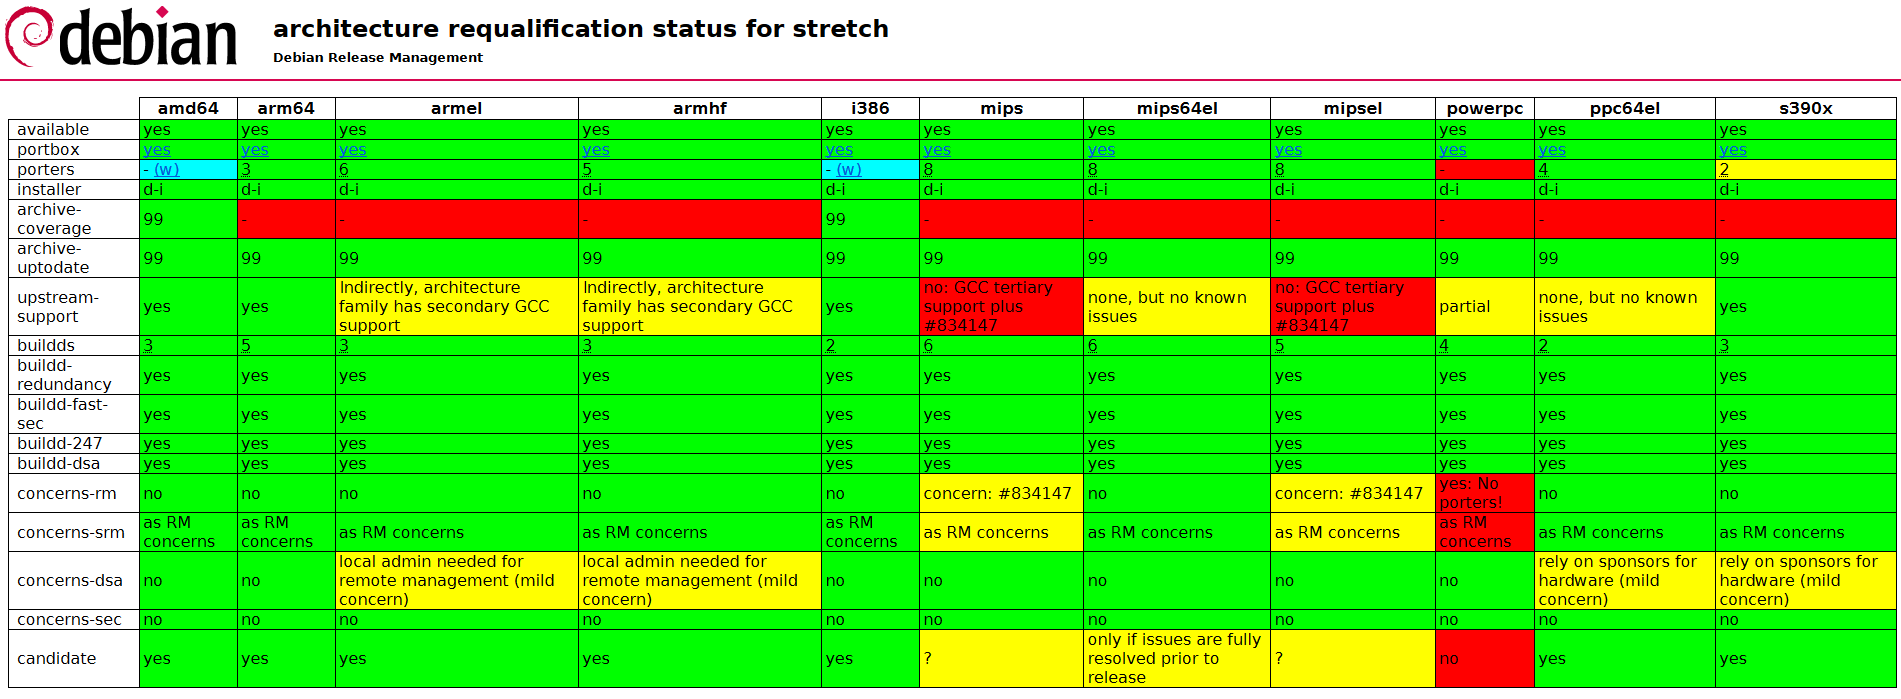
\includegraphics[width=1.0\hsize]{image201707/stretch-arch-requalification.png}
  % https://release.debian.org/stretch/arch_qualify.html
\end{center}

\end{frame}

\begin{frame}{Debian 9 について}% [containsverbatim]

テーマ\\
Juliette Taka Belin さんが作成した Soft waves を採用
\begin{center}
%%%  \includegraphics[width=0.8\hsize]{image201707/attachment_wallpaper.png}
\end{center}
% https://wiki.debian.org/DebianArt/Themes/softWaves
\end{frame}


\begin{frame}{Debian 9 について}% [containsverbatim]

ソフトウェア
\begin{itemize}
\item Linux カーネルは 4.9
\item ツールチェイン(GCC 6.3.0, binutils 2.28, glibc 2.24), LLVM 3.7.1, 3.8.1, 3.9.1
\item Perl 5.24.1, Python 2.7.13/3.5.3, Ruby 2.3.3, PHP 7.0.19, Go 1.7.4, OpenJDK 8
\item GNOME 3.22, KDE 5.8, Xfce 4.12.3, lxde 0.99.0, lxqt 0.11.1
\item MariaDB 10.1.23, PostgreSQL 9.6.3, sqlite 3.15
\item OpenSSL 1.1.0, GnuPG 2.1.18/1.4.21
\item クロスコンパイラがデフォルトでサポート
\item etc..
\end{itemize}

\end{frame}


\begin{frame}{Debian 9 について}% [containsverbatim]

パッケージの変更点
\begin{itemize}
\item iproute2が推奨、net-toolsは非推奨(例:ifconfig、arp、netstat、route)
\item firefox、thunderbirdという名称で提供
\item mysqlパッケージは提供されず、mariadbパッケージのみを提供
  \begin{itemize}
  \item jessieからアップグレードする場合は、自動でmariadbパッケージに置き換えられる
  \item データベースは自動変換されるが、元に戻せないこと、失敗することもありうることを想定し、データ保全は各自の責任で実施すること
  \end{itemize}
\item Xorg サーバはroot権限でなくユーザ権限で動作することが可能
\end{itemize}
\end{frame}


\begin{frame}{Debian 9 について}% [containsverbatim]

セキュリティ関係
\begin{itemize}
\item ウェブブラウザはセキュリティ更新が提供されるFirefoxおよびChromiumの利用を推奨
\item Firefox及びThunderbirdは、ESR版のセキュリティ更新を提供
\item libv8-3.14、nodejs、node-*はセキュリティ更新が提供されない
\item OpenSSLにおいて 3DES、RC4 暗号は TLS/SSL 通信には利用できない
\end{itemize}

\end{frame}


\begin{frame}{Debian 9 について}% [containsverbatim]

互換性
\begin{itemize}
\item ネットワークインタフェース名がenp1s1 (ethernet)、wlp3s0 (wlan)のように変更
  \begin{itemize}
  \item ただし、Debian 8 Jessieからアップグレードした場合は、eth0、wlan0といった昔の命名規則で据え置き
  \end{itemize}
\item OpenSSHは標準で旧式の暗号とSSH1プロトコルが無効
  \begin{itemize}
  \item 古いsshクライアントから接続できなくなる可能性があるため確認が必要
  \end{itemize}
\item X Window Systemのinputドライバがlibinputに変更
  \begin{itemize}
  \item Debian 8 jessieではevdevを採用
  \end{itemize}
\item Upstartは削除
  \begin{itemize}
  \item systemd(デフォルト)、SysVinit、OpenRCが利用可能
  \end{itemize}
\end{itemize}

\end{frame}


\begin{frame}{Debian 9 について}% [containsverbatim]

開発関連
\begin{itemize}
\item debhelper 10
  \begin{itemize}
  \item パラレルビルドがデフォルト化
%今までは明示的に指定する必要のあった\texttt{--parallel}オプションがデフォルト化。
  \item autoreconfをデフォルトで実行するように変更
%autotools を使っているソフトウェアでパッケージ作成時に再autoconf/automake する必要があるが、
%この際dh-autoreconf パッケージが必要だった。debhelper 10 からこの機能が取り込まれデフォルトで
%実行されるようになる。
  \item パッケージビルド時はdbgsymパッケージの生成をデフォルト化
    \begin{itemize}
    \item 生成したdbgsymパッケージは以下のapt-lineを指定して取得
    \item deb http://debug.mirrors.debian.org/debian-debug/ stretch-debug main
    \end{itemize}
  \item  dh\_installinit コマンドの \texttt{--restart-after-upgrade} オプションがデフォルト化
%init スクリプト を使うパッケージでアップグレード後にプログラムをリスタートする機能がデフォルト化。
%この機能が不要な場合は\texttt{--no-restart-after-upgrade}を指定する必要がある。
  \end{itemize}
\item 実行ファイルはデフォルトで PIE を有効にしてコンパイル及びリンクしている
\end{itemize}

\end{frame}


\begin{frame}{Debian 9 について}% [containsverbatim]

インストーラ
\begin{itemize}
\item GUIインストールがデフォルト
\item UEFIのセキュアブートは未対応
\item screen対応
\item multiarchのインストーラは、amd64をデフォルトでインストール
\item HTTPSミラーからパッケージのダウンロードが可能
\item 全バイナリパッケージを提供するISOファイルは、CDイメージを廃止
  \begin{itemize}
  \item DVDイメージ、blu-rayイメージのみの配布
  \item CDイメージは、netinst及びxfce4のみのデスクトップ環境を収録したCD一枚に収まる形でのみ提供
  \end{itemize}
\end{itemize}

\end{frame}


\begin{frame}{Debian 9 について}% [containsverbatim]

アップグレード方法
\begin{itemize}
\item リリースノートを一度読むことを推奨
\item apt-lineが"ftp://"の場合は、"http://"へ変更
\item 利用中のバージョンが古い場合はdebian-8へ順番にメジャーアップグレードする
  \begin{itemize}  
  \item メジャーバージョンの飛ばしアップグレードは非対応
  \end{itemize}
\item debian-8.8以降にアップグレードし、新しいkernelで起動するためrebootする
\item debian-9へのアップグレードはupgrade、dist-upgradeの2段階で行う
  \begin{itemize}
  \item apt-get update
  \item apt-get upgrade
  \item apt-get dist-upgrade
  \item reboot
  \end{itemize}
\end{itemize}

\end{frame}


\begin{frame}{Debian 9 について}% [containsverbatim]
  \begin{itemize}
    \item 何かおかしい動作や不具合を見つけた場合はbugreportをお願いします
  \end{itemize}
\end{frame}

%-----------------------

\section{Debian Updates}
\begin{frame}\begin{center}\Huge{Debian Updates}\end{center}\end{frame}


\begin{frame}{Debian Updates}% [containsverbatim]

\begin{itemize}[<+->]
\item 2017/01/14:  Updated Debian 8.7 released\\
\item 2017/05/06:  Updated Debian 8.8 released\\
\item 2017/07/22:  Updated Debian 8.9 released\\
  % https://lists.debian.org/debian-release/2017/07/msg00293.html
\ \\
   \small{}

\end{itemize}

\end{frame}


\begin{frame}{Debian Updates}% [containsverbatim]

\begin{itemize}[<+->]
\item 2017/4/15:  Debian Project Leader Elections 2017 投票締め切り\\
\ \\
   \small{2017年のDebianプロジェクトリーダー(DPL)を決める選挙が行われ、Chris Lambさんが選出されました。選挙における声明は、\url{https://www.debian.org/vote/2017/platforms/lamby} を参照。}

\end{itemize}

\end{frame}


\begin{frame}{Debian Updates}% [containsverbatim]

\begin{itemize}[<+->]
\item 2017/4/25:  Shutting down public FTP services\\
\ \\
\small{ftp://ftp.debian.org、ftp://security.debian.orgのFTPサービスが2017/11/1に停止する予定。HTTPサービスは継続するため、ftpを使っているユーザはapt-lineを"http://"に変更が必要。}

\end{itemize}

\end{frame}


\begin{frame}{Debian Updates}% [containsverbatim]

\begin{itemize}[<+->]
\item 2017/6/17:  Debian 9 「Stretch」 released\\
\item 2017/6/18:  Debian GNU/Hurd 2017 released\\
  % https://lists.debian.org/debian-hurd/2017/06/msg00017.html
\item 2017/7/22:  Debian 9.1 released\\
  % https://lists.debian.org/debian-release/2017/07/msg00294.html
\ \\
  \small{Debian 9 Stretchがリリースされた翌日に、sid(=unstable)のsnapshotとしてDebian GNU/Hurd 2017がリリースした。}

\end{itemize}

\end{frame}


\begin{frame}{Debian Updates}% [containsverbatim]

\begin{itemize}[<+->]
\item 2017/8/6-8/12:  debconf17\\
\ \\
  \small{debconf17をカナダ モントリオールで開催。webサイトでビデオを公開中。\url{https://debconf17.debconf.org/}}\\
\ \\
  \small{なお、debconf18は台湾 新竹市(Hsinchu) で 2018/7/29 - 8/4 に 開催する予定。}

\end{itemize}

\end{frame}


\section{日本語によるDebianの情報}
\begin{frame}\begin{center}\Huge{日本語によるDebianの情報}\end{center}\end{frame}

\begin{frame}{日本語によるDebianの情報}
\begin{itemize}
  \item Debian JP Project \\
      \url{http://www.debian.or.jp}
  \item 東京エリアDebian勉強会\\
      \url{http://tokyodebian.alioth.debian.org}
  \item 関西エリアDebian勉強会 \\
      \url{https://wiki.debian.org/KansaiDebianMeeting}
  \item Twitter \\
      \url{@debian_jp}
  \item G+ コミュニティ \\
      \url{https://plus.google.com/u/0/communities/106942835439686570073}
 
\end{itemize}
\end{frame}

%----------------

\section{今後のイベント}

\begin{frame}\begin{center}\Huge{今後のイベント}\end{center}\end{frame}

\begin{frame}{今後のイベント}

\begin{itemize}
\item 9/16 第155回東京エリアDebian勉強会
  \begin{itemize}
      \item 発表1: 初めてのキーサインパーティ
      \item 発表2: POMERA DM200にdebianをインストールしてみた
      \item \url{http://tokyodebian.alioth.debian.org/2017-09.html}
  \end{itemize}
\item 9/24 第127関西Debian勉強会
  \begin{itemize}
      % \item 福島区民センター  305号室
      \item \url{https://wiki.debian.org/KansaiDebianMeeting/20170924}
  \end{itemize}
\end{itemize}
\end{frame}

\begin{frame}{質問}
\begin{center}
何か質問はありますか?
\end{center}
\end{frame}

\end{document}

;;; Local Variables: ***
;;; outline-regexp: "\\([ 	]*\\\\\\(documentstyle\\|documentclass\\|emtext\\|section\\|begin{frame}\\)\\*?[ 	]*[[{]\\|[]+\\)" ***
;;; End: ***
